\documentclass[ucs, notheorems, handout]{beamer}

\usetheme[numbers,totalnumbers]{Statmod}
\usefonttheme[onlymath]{serif}
\setbeamertemplate{navigation symbols}{}

\usepackage[utf8x]{inputenc}
\usepackage[T2A]{fontenc}
\usepackage[russian]{babel}
\usepackage{tikz}
\usepackage{ragged2e}
\usepackage{amsthm}
\usepackage{wrapfig}
\usepackage{bm} %bold math
\usepackage{url}
\usepackage{dirtytalk} %for quotes
\usepackage{graphicx}
\usepackage{marginnote}
\usepackage{bm}
\usepackage[makeroom]{cancel}
\usepackage{algorithm2e}
\usepackage{pifont}
\usepackage{comment}
\newcommand{\sign}{\text{sign}}
\DeclareMathOperator*{\argmax}{arg\,max}
\DeclareMathOperator*{\argmin}{arg\,min}
\DeclareMathOperator{\rank}{rank}
\DeclareMathOperator{\diam}{diam}
\DeclareMathOperator{\ob}{Ob}
\DeclareMathOperator{\Hom}{Hom}
\DeclareMathOperator{\var}{Var}
\DeclareMathOperator{\bias}{Bias}
\newcommand{\betah}{\hat{\bm \beta}}
\newcommand{\betaa}{\bm{\beta}}
\newcommand{\epss}{\bm{\varepsilon}}
\newcommand{\E}{\mathrm{E}}
\newcommand{\D}{\mathrm{D}}
\newcommand{\XT}{{\bm{X}}^{\mathrm{T}}}
\newcommand{\X}{\bm{X}}
\renewcommand{\thealgocf}{}
\definecolor{asparagus}{rgb}{0.53, 0.66, 0.42}

\newtheorem{theorem}{Теорема}
\newtheorem{definition}{Определение}
\addto\captionsrussian{\renewcommand{\figurename}{Figure}}
\addto\captionsrussian{\renewcommand{\tablename}{Table}}

\title[Регрессия, регуляризация, отбор признаков]{%
     Регрессия, регуляризация, отбор признаков}

\author[Козак, Мехнин, Шкурат]{Михаил Козак, Павел Мехнин, Данил Шкурат}

\institute[Санкт-Петербургский Государственный Университет]{%
    \small
    Санкт-Петербургский государственный университет\\
    Кафедра статистического моделирования\\
    \vspace{1.25cm}
    Семинар по статистическому и машинному обучению}

\date[]{Санкт-Петербург, 2022}

\begin{document}
	
\begin{frame}[plain]
	\titlepage
	
	\note{Начнём.}
\end{frame}	

\begin{frame}
	\frametitle{Обучение с учителем}
	
	Обучение с учителем --- это направление машинного обучения, объединяющее алгоритмы и методы построения моделей на основе совокупности прецедентов (обучающей выборки), содержащих пары «известный вход — известный выход».
	
	\note{	}
	
	
\end{frame}



\begin{frame}
	\frametitle{Регрессия: формальная постановка}
	
	\begin{itemize}

	\item $X$ --- множество объектов, заданное своими признаками (точки $p$-мерного пространства)
	
	\item $Y$ --- множество ответов (действительные числа) 
	
	\item Предполагаем наличие неизвестной зависимости между объектами и ответами $y: X \to Y$
		  
	\item Обучающая выборка из множества объектов	$\{x_1, x_2, \dots, x_n\} \subset X$ и известных ответов (откликов) $y_i = y(x_i) \in Y, i = 1, \dots, n$ 
\end{itemize} 
		
	\textbf{Задача}:
	 
	 Найти $y^*: X \to Y$ --- отображение, приближающее неизвестную функцию $y$ на всём множестве $X$, то есть восстановить зависимость, способную для любого объекта выдать достаточно точный отклик.
	
\end{frame}

\begin{frame}
	\frametitle{Задача регрессии как задача оптимизации}
	
	\begin{itemize}
		\item $X_{n}=(x_{i},y_{i})_{i=1}^{n}$ --- обучающая выборка, $x_{i}\in\mathbb{R}^{p}$, $y_{i}\in\mathbb{R}$.
		\item $y_i = y(x_i) \in Y, i = 1, \dots, n$
		%\item $y_{i}=f^{\ast}(x_{i})+\varepsilon_{i}$, $i=1,\ldots,n$.
		\item Модель регрессии: параметрическое семейство функций $f(x,\beta)$, где $\beta\in B \subset\mathbb{R}^{p}$ --- вектор параметров модели.
		\item Средняя квадратичная ошибка (функционал качества, наиболее часто применяющийся в задачах регрессии):
		\begin{equation*}
			Q(\theta,X_{n})=
			\sum_{i=1}^{n}
			(f(x_{i},\beta)-y_{i})^{2}.
		\end{equation*}
		\item Задача обучения по МНК --- задача минимизации
		\begin{equation*}
			Q(\beta,X_{n})
			\rightarrow
			\min_{\beta\in B}.
		\end{equation*}
	\end{itemize}
\end{frame}

\begin{frame}
	\frametitle{Линейная регрессия: постановка}
	Модель:	 $\bm y = \X \betaa + \epss$
	\begin{itemize}
		\item $\bm y \in \mathbb R^n$ --- вектор ответов,  $\epss \in \mathbb R^n$ --- вектор ошибок, $\mathbb{E}\epss = \bm 0$
		\item $\X \in \mathbb R^{n \times p}$ --- матрица данных 
	
		\item $\betaa \in \mathbb R^p$ --- вектор параметров модели
	\end{itemize}

	\begin{figure}[]
	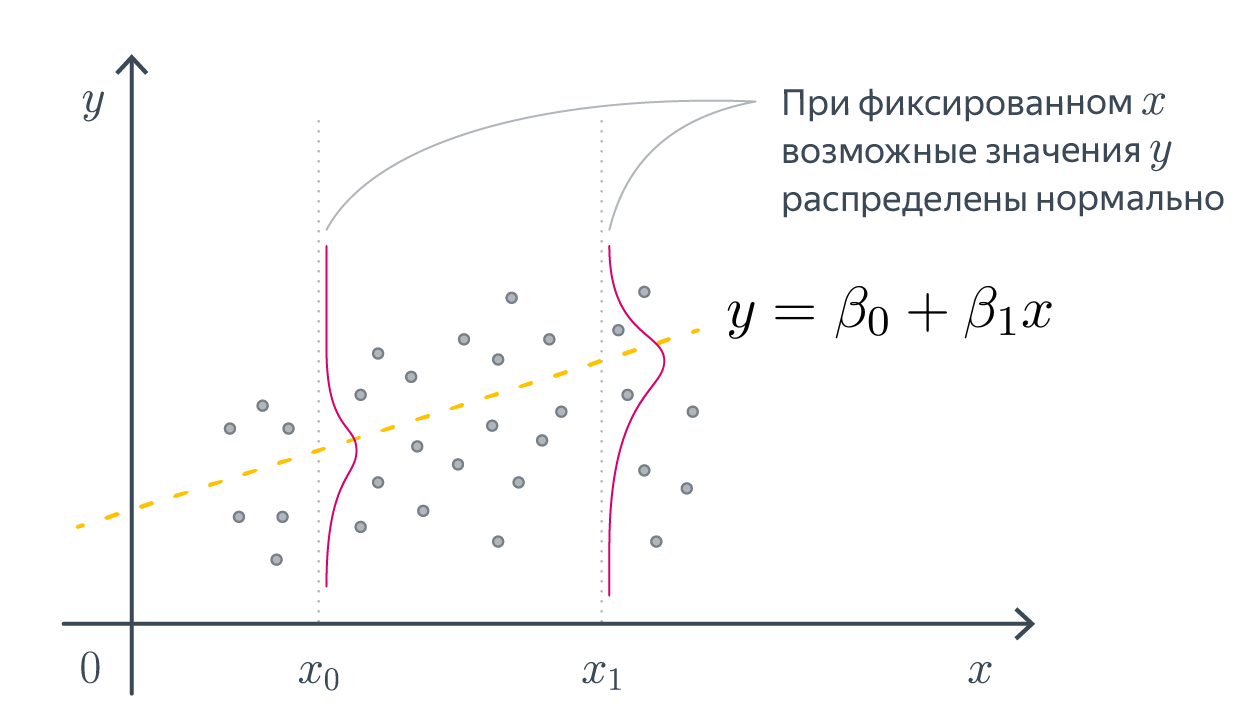
\includegraphics[width=0.8\textwidth]{Prob_regression1.png}
\end{figure}


	
	Решение задачи линейной регрессии --- вектор $\betah$. 
	


	
%	Исходная модель не обязательно линейна: ищем наилучшую аппроксимацию в подпространстве столбцов $\X$.
	
	\note{
		Предположения о модели:
		
		1. Матрица плана неслучайна
		
		2. Матрица $\XT\X$ невырожденна 
		
		3. $\E \varepsilon_i = 0,\, \E \varepsilon_i^2 = \sigma^2 < +\infty,\,  \E \varepsilon_i \varepsilon_j = 0$
	}
\end{frame}





\begin{comment}

\begin{frame}
	\frametitle{Задача регрессии как задача оптимизации}
	\begin{itemize}
		\item $\X \in \mathbb R^{n \times p}$ --- матрица данных
		\item $\bm y \in \mathbb R^n$ --- вектор ответов
		\item $\betaa \in \mathbb R^d$ --- вектор параметров 
		\item $\bm \varphi(\X, \betaa) := (\varphi(\mathbf x_1, \betaa),\ldots, \varphi(\mathbf x_n, \betaa) )^\mathrm T$ --- функция от выборки и параметров	\item $\mathcal L(\bm \varphi(\X, \betaa), \bm y)$ ---  функция потерь
	\end{itemize}
	Решение задачи регрессии --- вектор коэффициентов $\betah$. 
	
		$$\betah = \argmin_{\betaa}{\mathcal L(\bm \varphi(\X, \betaa), \bm y)}$$

	
	\note{
		Пока что представляем для примера, что функция потерь квадратичная, стандартная, с другими мы ещё не встретились. Так как успешное решение нашей задачи эквивалентно нахождению минимума указанного функционала, становится важным его вид. В случае линейной регрессии и квадратичной функции потерь у этого минимума есть явный вид, однако при выборе более сложных функций потерь нахождение этого минимума становится непростой задачей.
	}
\end{frame}


\begin{frame}
	\frametitle{Линейная регрессия}
	
	Введем матричные обозначения:
\begin{itemize}
	\item  $\mathbb{X} = [X_1, \ldots, X_p]$, где $X_i = (x_{1i}, \ldots, x_{ni})^{T}$, $i = 1, \ldots, p$
	\item  $Y=(y_{1},\ldots,y_{n})^{\mathrm{T}}$ $\mathcal{E}=(\varepsilon_{1},\ldots,\varepsilon_{n})^{\mathrm{T}}$, 
	\item  $B=(\beta_{1},\ldots,\beta_{p})$ --- вектор параметров модели.
\end{itemize}
	
	Модель линейной регрессии в матричной форме:
	\begin{equation*}
		Y=\beta_{1}X_{1}+\cdots+\beta_{p}X_{p}+\mathcal{E}
		=
		\mathbb{X}B+\mathcal{E}.
	\end{equation*}
	
	Задача оптимизации принимает вид: 
	\begin{equation*}
		Q(B,X)=
		||Y-\mathbb{X}B||^{2}
		\rightarrow
		\min_{B}.
	\end{equation*}
	

\end{frame}

\end{comment}
\begin{frame}
	\frametitle{Линейная регрессия}
	
	Задача оптимизации (с квадратичной функцией потерь):
	
	$$\betah = \argmin_{\betaa}{\|\bm y - \bm X \betaa\|^2_2}$$
	
	Полученную оценку называют оценкой по методу наименьших квадратов. Она имеет явный вид:
	
 $$\betah_{\text{МНК}}=(\bm{X}^{\mathrm{T}}\bm{X})^{-1}\bm{X}^{\mathrm{T}} \bm y=\bm{X}^{-}\bm y$$ 
	$$\hat{\bm y}=\bm{X}\betah_{\text{МНК}}$$
	
	Теорема Гаусса--Маркова утверждает, что $\betah_{\text{МНК}}$ имеет наименьшую дисперсию среди всех несмещённых оценок (best linear unbiased estimate --- BLUE).
	
	
	Достаточно быстро вычисляется  посредством применения сингулярного разложения.
	
	
\end{frame}

\begin{comment}

\begin{frame}
	\frametitle{Множественная линейная регрессия}
	Пусть $\mathbb{X}=\mathbb{V}\mathbb{\Lambda}\mathbb{U^{\mathrm{T}}}$ --- сингулярное разложение $\mathbb{X}$.
	\begin{itemize}
		\item Тогда псевдообратную к $\mathbb{X}$ матрицу легко записать в виде
		\begin{equation*}
			\mathbb{X}^{-}
			=
			\mathbb{U}\mathbb{\Lambda}^{-1}\mathbb{V}^{\mathrm{T}}
			=
			\sum_{j=1}^{p}
			\frac{1}{\sqrt{\lambda_{j}}}
			U_{j}V_{j}^{\mathrm{T}}.
		\end{equation*}
		\
	\end{itemize}
\end{frame}

\end{comment}

\begin{frame}
	\frametitle{МНК-оценка: вычислительный взгляд}
	
		Сингулярное разложение: $\X = \bm V \bm D \bm U^\mathrm T$
		\begin{itemize}
			\item $\bm V$ и $\bm U$ --- ортогональные, $\bm D$ --- диагональная
			\item $\bm V = (V_1, V_2, \ldots, V_n) \in \mathbb R^{n\times n}$, $V_i$ --- с.\,векторы $\X \XT$
			\item $\bm U = (U_1, U_2, \ldots, U_n) \in \mathbb R^{p\times n}$, $U_i$ --- с.\,векторы $\XT \X$
			\item $\bm D = \mathrm{diag}(\sqrt{\lambda_1}, \ldots,\sqrt{\lambda_n})$, $\lambda_j \geqslant 0$ --- с.\,значения $\XT \X$
		\end{itemize}
		
		Подставим в формулу для $\betah_{\text{МНК}}$ вместо матрицы $\X$ её сингулярное разложение и получим
		$$
\betah = (\XT \X)^{-1}\XT \bm y = (\bm U \bm D \bm V^\mathrm{T} \bm V \bm D \bm U^\mathrm{T})^{-1} \bm U \bm D \bm V^\mathrm{T} \bm y = \bm U \bm D^{-1} \bm V^\mathrm{T} \bm y,
$$
		где $\bm D^{-1} = \mathrm{diag} (1/\sqrt{\lambda_1}, \ldots, 1/\sqrt{\lambda_n})$.
		 
		\begin{equation*}
			\betah_{\text{МНК}}
			=
			\sum_{j=1}^{p}
			\frac{1}{\sqrt{\lambda_{j}}}
			U_{j}(V_{j}^{\mathrm{T}} \bm y)
		\end{equation*}
		

	\note{	
	}

\end{frame}
	

\begin{frame}
	\frametitle{Мультиколлинеарность признаков}
	
	Пусть матрица данных содержит несколько сильно коррелированных признаков (есть $\lambda_{j}\rightarrow0$).
	
	Что будет происходить в таком случае с МНК-оценкой?
	\begin{itemize}
		\item Решение $\hat{\bm \beta}$  неустойчиво 
		\item Решение неинтерпретируемо,  $||\hat{\bm \beta}||\rightarrow\infty$
		\item Высокая дисперсия у $\hat{\bm \beta} \to$ высокая MSE
		\item Ответы на контрольной выборке неустойчивы (переобучение)
	\end{itemize}
	\textbf{Способы решения проблемы:}
	\begin{itemize}
		\item Регуляризация
		\item Уменьшение числа признаков (отбор признаков)
		\item Преобразование признаков (анализ главных компонент)
	\end{itemize}
\end{frame}

\begin{frame}
	\frametitle{Регуляризация}
	Хорошая оценка $\betah$ должна иметь низкую среднеквадратическую ошибку 
	\begin{equation*}
		\label{eq:mse}
		\mathbb{E}(\betaa - \betah)^2 = \underbrace{\mathbb D \betah}_{\text{дисперсия}} + \underbrace{(\mathbb E \betah - \betaa)^2}_{\text{смещение}}.
	\end{equation*}

	Несмещенная МНК-оценка не гарантирует минимизацию всей $\mathrm{MSE}$,
	т.к. может иметь большую дисперсию (если матрица $\bm X$ близка к вырожденной).
	
	
	Введение небольшого смещения в оценке может привести к уменьшению дисперсии и тем самым уменьшению $\mathrm{MSE}_{\text{test}}$.

	
\end{frame}


\begin{comment}

\begin{frame}
	\frametitle{Борьба с мультиколлинеарностью}
		В ряде случаев (признаков больше чем объектов, коррелирующие признаки) оптимизационная задача $Q(w) \to \min$ может иметь бесконечное число решений, большинство которых являются переобученными и плохо работают на тестовых данных.
		
		Пусть в выборке есть линейно зависимые признаки. Это по определению означает, что $\exists \, \bm v$, что $\forall  x$ выполнено $\langle \bm v, \bm x \rangle = 0$.
		Допустим, мы нашли оптимальный вектор весов $w$ для линейного классификатора.
		Но тогда классификаторы с векторами $w + \alpha v$ будут давать точно такие же ответы на всех объектах, поскольку
		$$
		\langle w + \alpha v, x \rangle = \langle w,x \rangle + \alpha \langle v,x \rangle = \langle w,x \rangle
		$$
		
		
		Это значит, что метод оптимизации может найти решение со сколько угодно большими весами. 
		
	\note{
		Такие решения не очень хороши, поскольку классификатор будет чувстви-
		телен к крайне маленьким изменениям в признаках объекта, а значит, переобучен.
		Мы уже знаем, что переобучение нередко приводит к большим значениям ко-
		эффициентов. Чтобы решить проблему, добавим к функционалу регуляризатор, ко-
		торый штрафует за слишком большую норму вектора весов:
	}
\end{frame}



\begin{frame}
	\frametitle{Борьба с мультиколлинеарностью}
	\begin{centering}
		\textbf{Мультиколлинеарность ($\XT \X$ плохо обусловлена) влечёт}
	\end{centering}
	
	\begin{itemize}
		\item Неустойчивость решения
		\item Высокая дисперсия у $\betah$ $\Rightarrow$ высокая MSE
	\end{itemize}
	\vspace{0.5cm}
	\begin{centering}
		\textbf{Возможные решения проблемы мультиколлинеарности}
	\end{centering}
	
	
	\begin{itemize}
		\item Регуляризация
		\item Уменьшение числа признаков (отбор признаков)
		\item Преобразование признаков (анализ главных компонент)
	\end{itemize}
	\note{
	}
\end{frame}
	


\begin{frame}
	\frametitle{Регуляризация}

\begin{itemize}
	\item  $\mathrm{MSE}_{\mathrm{test}}$ зависит от дисперсии оценки $\hat{f}$ и ее смещения.
	\item Когда связь между откликом и предикторами (почти) линейна, оценки по МНК обладают (почти) нулевым смещением, но при этом могут иметь большую дисперсию. 

	\item Чем больше дисперсия оценки $\hat{B}$, тем больше дисперсия $\hat{f}$. 
	\item Когда матрица $\mathbb{X}$ близка к вырожденной, дисперсия $\hat{B}$ становится большой и $\mathrm{MSE}_{\mathrm{test}}$ увеличивается.  
	\item При $p>n$ или при полностью коллинеарных признаках оценки по МНК не имеют уникального решения.
	\item Введение небольшого смещения в оценке может привести к уменьшению дисперсии и тем самым уменьшению $\mathrm{MSE}_{\text{test}}$.
\end{itemize}
	
	\note{
		
	}
\end{frame}	
\end{comment}


\begin{frame}
	\frametitle{Регуляризация. Гребневая регрессия}

\begin{itemize}
	\item Вводим штраф за увеличение нормы вектора $\bm \beta$ и переходим к минимизации следующей функции:
	\begin{equation*}
		Q_{\tau}(\bm \beta)
		=
		||\bm{X} \bm \beta-\bm y||^{2}
		+
		\tau||\bm \beta||^{2}
		\rightarrow\min_{\bm \beta},
	\end{equation*}
	где $\tau$ --- неотрицательный параметр регуляризации.
	\item В развернутом виде задача оптимизации записывается так:
	\begin{equation*}
		\sum_{i=1}^{n}
		\left(
		y_{i}
		-
		\sum_{j=1}^{p}\beta_{j}x_{ij}
		\right)^{2}
		+
		\tau\sum_{j=1}^{p}\beta_{j}^{2}
		\rightarrow\min_{\bm \beta}.
	\end{equation*}
	\item Решение:
	\begin{equation*}
		\hat{\bm \beta}_{\text{ridge}}
		=
		(\bm{X}^{\mathrm{T}}\bm{X}+\tau\bm{I}_{p})^{-1}\bm{X}^{\mathrm{T}} \bm y.
	\end{equation*}
\end{itemize}

\end{frame}



\begin{frame}
	\frametitle{Регуляризация. Гребневая регрессия}

	
	Используем SVD и получим
	$$\betah_{\text{ridge}} = \sum_{i = 1}^n \frac{\lambda_j}{\lambda_j + \tau} U_j(V_j^\mathrm T\bm y)$$
	
	Отделили знаменатель от нуля. Устойчивость вычислений повышается.
	
	Преимущество SVD разложения: можно подбирать параметр $\tau$ вычислив SVD только один раз.
	
Чем больше коэффициент регуляризации $\tau$, тем устойчивее решение, но больше смещение. 

Когда $\tau = 0$, то гребневая регрессия совпадает с обычной регрессией, но при $\tau \rightarrow \infty$ коэффициенты регрессии стремятся к нулю.
	
	\note{
		
	}
\end{frame}


\begin{comment}


\begin{frame}
	\frametitle{Гребневая регрессия. Дисперсия}
	$$\mathrm{MSE} = \E(\betaa - \betah)^2 = \underbrace{\mathrm D \betah}_{\text{дисперсия}} + \underbrace{(\mathrm E \betah - \betaa)^2}_{\text{смещение}}$$
	
	
	\textit{Смещение} контролируется параметром $\tau$ и возрастает с его увеличением.
	
	\textit{Что с дисперсией?}
	
	\begin{itemize}
		\item $\betah_{\text{ridge}} = \sum_{i = 1}^n \frac{\sqrt{\lambda_j}}{\lambda_j + \tau} U_j(V_j^\mathrm T\bm y)$
		\item $\lambda_j$ убывают
		\item $\frac{\sqrt{\lambda_j}}{\lambda_j + \tau}$ штрафуют компоненты с наименьшей дисперсией
		\item  $\D \betah$ уменьшается $\, \Rightarrow \,$  MSE $\downarrow$
	\end{itemize}
	
	
	\note{
		
	}
\end{frame}

\end{comment}


\begin{frame}
	\frametitle{Гребневая регрессия. Выбор параметра}
	
	
			\begin{figure}[]
				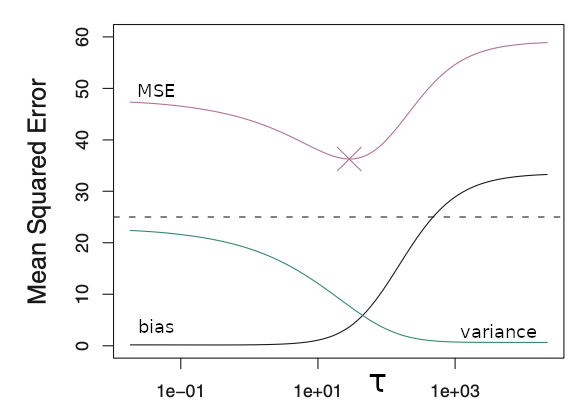
\includegraphics[width=1\textwidth]{ridge2.png}
			\end{figure}

	\note{
		
	}
\end{frame}

\begin{frame}
	\frametitle{Подбор параметра $\tau$ }
	
	\textbf{Скользящий контроль}:%см слайд 41 в 08 короба
	\begin{itemize}
		\item выбираем сетку значений $\tau$;
		\item вычисляем ошибку кросс-проверки для каждого значения $\tau$;
		\item выбираем $\tau$ с наименьшим значением ошибки кросс-проверки;
		\item перестраиваем модель со всеми наблюдениями с выбранным значением $\tau$.
	\end{itemize}
	
	\textbf{Эвристика }
	
	Скользящий контроль --- вычислительно трудоёмкая процедура. Известна практическая рекомендация брать брать $\tau$ в отрезке $[0.1, 0.4]$, если столбцы матрицы $\bm{X}$ заранее стандартизованы.
	
\end{frame}


\begin{frame}
\frametitle{Лассо регуляризация}

\begin{itemize}
	\item В качестве штрафа за увеличение нормы вектора $\bm \beta$ используется его $l_{1}$-норма.
	\item Метод LASSO решает следующую задачу минимизации:
	\begin{equation*}
		||\bm{X} \bm \beta - \bm y||_{2}^{2}
		+
		\tau||\bm \beta||_{1}^{2}
		\rightarrow\min_{\bm \beta},
	\end{equation*}
	где $\tau$ --- неотрицательный параметр регуляризации.
	\item Задача оптимизации в развернутом виде:
	\begin{equation*}
		\sum_{i=1}^{n}
		\left(
		y_{i}
		-
		\sum_{j=1}^{p}\beta_{j}x_{ij}
		\right)^{2}
		+
		\tau\sum_{j=1}^{p}|\beta_{j}|
		\rightarrow\min_{\beta_{1},\ldots,\beta_{p}}.
	\end{equation*}
\end{itemize}
\end{frame}

\begin{frame}
	\frametitle{Регуляризация. Lasso}
	
	
	Задачу lasso-оптимизации можно переписать в форме с ограничениями: %(метод множителей Лагранжа)
	\begin{equation*}%\label{eq:lasso_constr}
		\begin{cases}
			\sum_{i=1}^{n}
			\left(
			y_{i}
			-
			\sum_{j=1}^{p}\beta_{j}x_{ij}
			\right)^{2}
			\to
			\min_{\beta_{1},\ldots,\beta_{p}},\\
			\sum_{j=1}^{p}|\beta_{j}|\leq\ae,
		\end{cases}
	\end{equation*}
	где $\ae=1/\tau$.

		%$$
		%\betah_{\text{Lasso}}(\lambda) = \argmin_{\betaa}{\|\bm y - \X\betaa\|^2_2 %\text{,  } \|\betaa\|^2_1 \leqslant \lambda}
		%$$

	\textbf{
		Особенности:
	}
	\begin{itemize}
		\item Уменьшение MSE
		\item Интерпретируемость результатов
		\item Быстрое вычисление $\betah_\text{Lasso}(\tau)$
		\item Выбор параметра: кросс-валидация
	\end{itemize}
	\note{
	}
\end{frame}




\begin{frame}
	\frametitle{Сравнение гребневой регрессии и Лассо}
	\begin{figure}[]
		\center{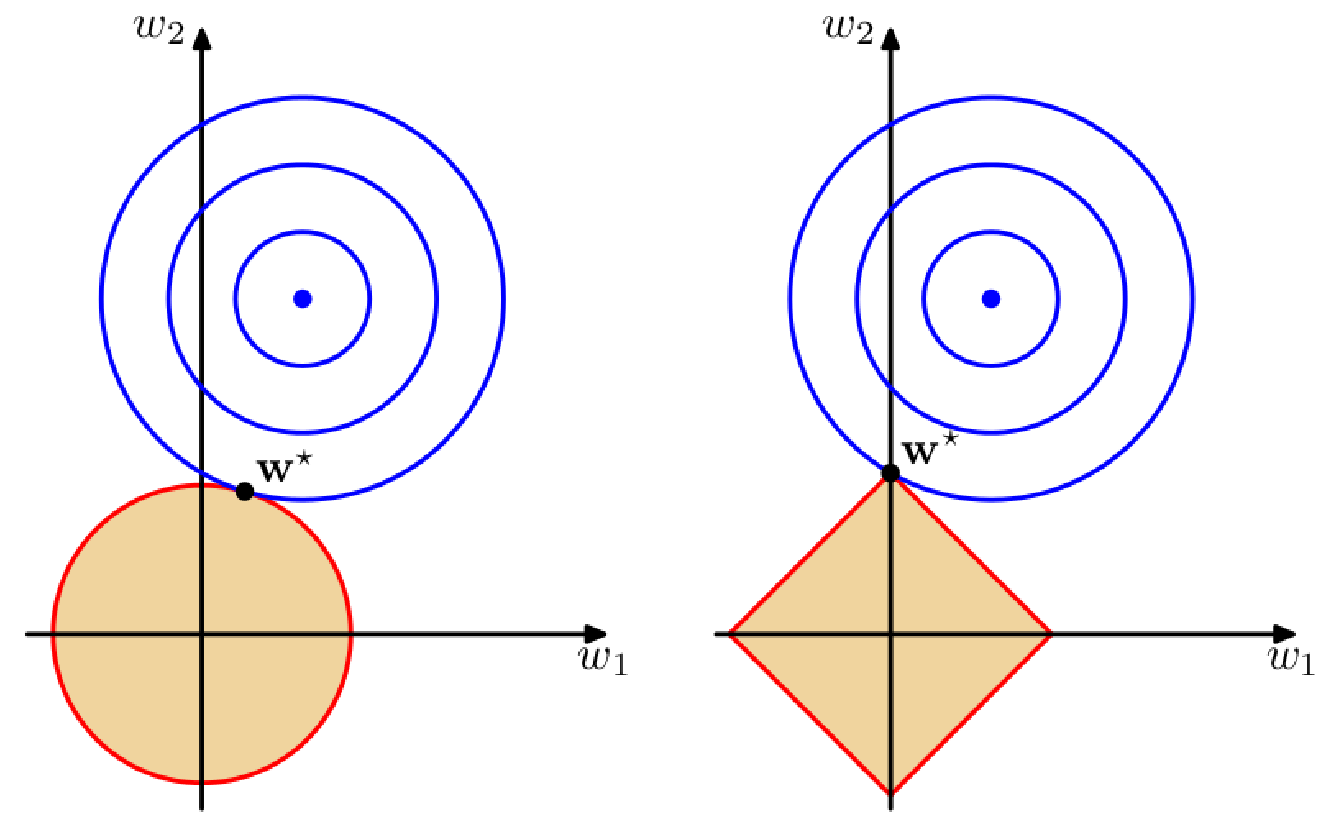
\includegraphics[width=0.8\linewidth]{reg.eps}}
		
		Синие линии уровня функционала качества (синяя точка --- безусловный минимум, который достигается на МНК решении). Оранжевая зона --- ограничения, задаваемые L2 и L1-регуляризаторами. Чёрная точка --- минимум целевой функции при заданном ограничении.
	\end{figure}
\end{frame}


\begin{frame}
	\frametitle{Сравнение гребневой регрессии и Лассо}
	
	\vspace{0.8cm}
	\begin{itemize}
		\item Оба метода успешно решают проблему мультиколлинеарности
		\item Гребневая регрессия использует все признаки
		\item Лассо производит отбор признаков, что предпочтительнее, если среди признаков есть шумовые или измерения признаков связаны с ощутимыми затратами.
		\item С помощью кросс-валидации можно определить какой подход лучше для конкретных данных.
	\end{itemize}
\end{frame}

\begin{frame}
	\frametitle{Elastic net regularization}
	Решается задача оптимизации
	\begin{equation*}
		||\bm y-\bm {X} \bm \beta||_{2}^{2} + \tau_{1}||\bm \beta||_{1}^{2}+\tau_{2}||\bm \beta||_{2}^{2}
		\rightarrow\min_{\bm \beta}.
	\end{equation*}
	\begin{itemize}
		\item[\checkmark] Elastic net --- это комбинация методов Lasso и Ridge:
		\begin{itemize}
			\item Когда $\tau_1 = 0$: Ridge регрессия
			\item Когда $\tau_2 = 0$: Lasso регрессия
		\end{itemize}
		\item[\checkmark] Elastic net в целом лучше, чем Lasso при наличии коррелированных признаков
		\item[\checkmark] В отличие от Ridge регрессии, когда $p > n$, Elastic net может учитывать более $n$ переменных

	\end{itemize}
\end{frame}


\begin{frame}
	\frametitle{Отбор признаков. BSS, Forward, Backward}
	
	\textbf{Алгоритм полного перебора (Best Subset Selection)}
		
		
		Преимущества:
		\begin{itemize}
		\item[\checkmark]простота реализации
		\item[\checkmark]гарантированный результат
		\item[\checkmark] эффективен, когда информативных признаком немного ($\le 5$) и общее количество признаков также не велико ($\le 20 \dots 100$)
	\end{itemize}

		Недостатки:
		\begin{itemize}
		\item[\ding{55}]в общем случае очень долго: $O(2^p)$. Например, для p = 20: $2^p = 1,048,576$ моделей
		\item[\ding{55}]чем больше перебирается вариантов, тем больше перобучение
		
\end{itemize}
		Решение: эвристические алгортмы сокращенного перебора
		
\end{frame}
\begin{frame}
	\frametitle{Отбор признаков. BSS, Forward, Backward}
	
	\textbf{Жадные (greedy) алгоритмы}
	
	
	\begin{itemize}
		\item Forward Stepwise Selection 
		
		
		Начинаем со свободного члена, потом добавляем на каждом шаге предиктор, который
		максимально уменьшает ошибку. 
		
		Подмножества получаются вложенные ---  для $p = 20$: $p (p + 1) / 2 = 210$ моделей.
		
		\item Backward Stepwise Selection
		
		Начинаем с полной регрессии и на каждом шаге убираем предиктор, который оказывает меньше всего влияния на ошибку.
	\end{itemize}

\end{frame}

\end{document}

